

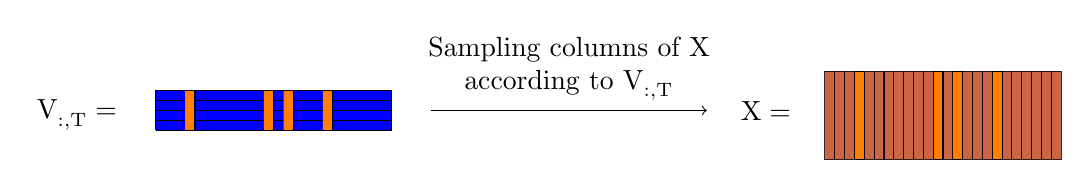
\begin{tikzpicture}[scale = 0.5]

  % draw line and angle
%  \draw 
%     pic [draw,angle radius=4mm,angle eccentricity=1.5, "$\theta$" font=\scriptsize] {angle=v2--v1--v3};

\begin{scope}[xshift=-65mm]



\draw [fill=blue, opacity=1] (0.5,3.25) -- (6.5,3.25) -- (6.5,3.5) -- (0.5,3.5) -- (0.5,3.25);
\draw [fill=blue, opacity=1] (0.5,3) -- (6.5,3) -- (6.5,3.25) -- (0.5,3.25) -- (0.5,3);
\draw [fill=blue, opacity=1] (0.5,2.75) -- (6.5,2.75) -- (6.5,3) -- (0.5,3) -- (0.5,2.75);
\draw [fill=blue, opacity=1] (0.5,2.5) -- (6.5,2.5) -- (6.5,2.75) -- (0.5,2.75) -- (0.5,2.5);


\draw [fill=orange, opacity=1] (1.25,2.5) -- (1.25,2.5) -- (1.5,2.5) -- (1.5,3.5) -- (1.25,3.5);
\draw [fill=orange, opacity=1] (3.25,2.5) -- (3.25,2.5) -- (3.5,2.5) -- (3.5,3.5) -- (3.25,3.5);
\draw [fill=orange, opacity=1] (3.75,2.5) -- (3.75,2.5) -- (4,2.5) -- (4,3.5) -- (3.75,3.5);
\draw [fill=orange, opacity=1] (4.75,2.5) -- (4.75,2.5) -- (5,2.5) -- (5,3.5) -- (4.75,3.5);


 \draw  (-1.5,2.25)  node [above] {$\bm{\mathrm{V}}_{:,\mathrm{T}}^{\Tran}=$} ;
\end{scope}

\begin{scope}[xshift=10mm]


\draw [fill=Bittersweet, opacity=0.8] (16,4) -- (15.75,4) -- (15.75,1.75) -- (16,1.75) -- (16,4);
\draw [fill=Bittersweet, opacity=0.8] (15.75,4) -- (15.5,4) -- (15.5,1.75) -- (15.75,1.75) -- (15.75,4);

\draw [fill=Bittersweet, opacity=0.8] (15.5,4) -- (15.25,4) -- (15.25,1.75) -- (15.5,1.75) -- (15.5,4);
\draw [fill=Bittersweet, opacity=0.8] (15.25,4) -- (15,4) -- (15,1.75) -- (15.25,1.75) -- (15.25,4);
\draw [fill=Bittersweet, opacity=0.8] (15,4) -- (14.75,4) -- (14.75,1.75) -- (15,1.75) -- (15,4);
\draw [fill=Bittersweet, opacity=0.8] (14.75,4) -- (14.5,4) -- (14.5,1.75) -- (14.75,1.75) -- (14.75,4);
\draw [fill=orange, opacity=1] (14.5,4) -- (14.25,4) -- (14.25,1.75) -- (14.5,1.75) -- (14.5,4);
\draw [fill=Bittersweet, opacity=0.8] (14.25,4) -- (14,4) -- (14,1.75) -- (14.25,1.75) -- (14.25,4);
\draw [fill=Bittersweet, opacity=0.8] (14,4) -- (13.75,4) -- (13.75,1.75) -- (14,1.75) -- (14,4);
\draw [fill=Bittersweet, opacity=0.8] (13.75,4) -- (13.5,4) -- (13.5,1.75) -- (13.75,1.75) -- (13.75,4);
\draw [fill=orange, opacity=1] (13.5,4) -- (13.25,4) -- (13.25,1.75) -- (13.5,1.75) -- (13.5,4);
\draw [fill=Bittersweet, opacity=0.8] (13.25,4) -- (13,4) -- (13,1.75) -- (13.25,1.75) -- (13.25,4);
\draw [fill=orange, opacity=1] (13,4) -- (12.75,4) -- (12.75,1.75) -- (13,1.75) -- (13,4);

\draw [fill=Bittersweet, opacity=0.8] (12.75,4) -- (12.5,4) -- (12.5,1.75) -- (12.75,1.75) -- (12.75,4);
\draw [fill=Bittersweet, opacity=0.8] (12.5,4) -- (12.25,4) -- (12.25,1.75) -- (12.5,1.75) -- (12.5,4);
\draw [fill=Bittersweet, opacity=0.8] (12.25,4) -- (12,4) -- (12,1.75) -- (12.25,1.75) -- (12.25,4);
\draw [fill=Bittersweet, opacity=0.8] (12,4) -- (11.75,4) -- (11.75,1.75) -- (12,1.75) -- (12,4);

\draw [fill=Bittersweet, opacity=0.8] (11.75,4) -- (11.5,4) -- (11.5,1.75) -- (11.75,1.75) -- (11.75,4);
\draw [fill=Bittersweet, opacity=0.8] (11.5,4) -- (11.25,4) -- (11.25,1.75) -- (11.5,1.75) -- (11.5,4);
\draw [fill=Bittersweet, opacity=0.8] (11.25,4) -- (11,4) -- (11,1.75) -- (11.25,1.75) -- (11.25,4);
\draw [fill=orange, opacity=1] (11,4) -- (10.75,4) -- (10.75,1.75) -- (11,1.75) -- (11,4);
\draw [fill=Bittersweet, opacity=0.8] (10.75,4) -- (10.5,4) -- (10.5,1.75) -- (10.75,1.75) -- (10.75,4);
\draw [fill=Bittersweet, opacity=0.8] (10.5,4) -- (10.25,4) -- (10.25,1.75) -- (10.5,1.75) -- (10.5,4);
\draw [fill=Bittersweet, opacity=0.8] (10.25,4) -- (10,4) -- (10,1.75) -- (10.25,1.75) -- (10.25,4);


\draw  (8.5,2.5)  node [above] {$\bm{\mathrm{X}} = $} ;
\end{scope}


\draw [->] (1,3) --  (4.5,3)  node [above] {} --  (8,3);

\draw  (4.5,3)  node [above , align=center] {Sampling columns of $\bm{\mathrm{X}}$\\ according to $\bm{\mathrm{V}}_{:,\mathrm{T}}^{\Tran}$} ;



% \draw [->] (-9.5,3) --  (-7.5,3)  node [above] { $\Prb(T)$} --  (-5,3);

% \draw [->] (3,3) --  (5,3)  node [above] { $\Prb(S|T)$} --  (7.5,3);


% \draw  (-7.5,4.25)  node [above] {Step 1} ;

% \draw  (5,4.25)  node [above] {Step 2} ;

%\draw  (23,2)  node [above] {Complexity } ;

\end{tikzpicture}
